\documentclass[lettersize,journal]{IEEEtran}
\usepackage{algorithm}
\usepackage{array}
\usepackage[caption=false,font=normalsize,labelfont=sf,textfont=sf]{subfig}
\usepackage{textcomp}
\usepackage{stfloats}
\usepackage{url}
\usepackage{verbatim}
\usepackage{graphicx}
\usepackage{cite}
\hyphenation{op-tical net-works semi-conduc-tor IEEE-Xplore}
\usepackage{amsmath,amssymb,amsfonts,amsthm,bm,mathtools}
\usepackage{algorithmic}
\usepackage{xcolor}
\usepackage{multirow}
\usepackage{booktabs}
\graphicspath{{fig/}}
\usepackage{siunitx}
\usepackage[hidelinks]{hyperref}

% ---- shared theorem counter (all theorem-family types share one counter) ----
\newtheorem{theo}{Theorem}
\newtheorem{lemma}[theo]{Lemma}
\newtheorem{prop}[theo]{Proposition}
\newtheorem{coro}[theo]{Corollary}
\newtheorem{defi}[theo]{Definition}
\newtheorem{conj}[theo]{Conjecture}
\newtheorem{propprime}[theo]{Proposition}
\theoremstyle{remark}
\newtheorem{rem}[theo]{Remark}

% ---- proof inclusion toggle ----
\newif\ifincludeproofs

% ---- handy macros ----
\newcommand{\R}{\mathbb{R}}
\newcommand{\Z}{\mathbb{Z}}
\newcommand{\E}{\mathbb{E}}
\newcommand{\Var}{\operatorname{Var}}
\newcommand{\Cov}{\operatorname{Cov}}
\newcommand{\tr}{\operatorname{tr}}
\newcommand{\rank}{\operatorname{rank}}
\newcommand{\supp}{\operatorname{supp}}
\newcommand{\diag}{\operatorname{diag}}
\newcommand{\MP}{\mathrm{MP}}
\newcommand{\MixPoi}{\operatorname{MixPoi}}
\newcommand{\Poi}{\operatorname{Poi}}
\newcommand{\ESS}{\mathrm{ESS}}
\newcommand{\deff}{d_{\mathrm{eff}}}
\newcommand{\floor}[1]{\lfloor #1 \rfloor}
\newcommand{\fracp}[1]{\operatorname{frac}(#1)}
\begin{document}

\title{Spectral Costs of Multinomial and Residual Resampling in High-Dimensional Particle Ensembles: A Free-Probability Analysis}

\author{Deming~SONG,~\IEEEmembership{Student Member,~IEEE,}%
\thanks{Deming SONG is with the Faculty of Applied Sciences, Macao Polytechnic University, Macao, China (e-mail: p2514650@mpu.edu.mo).}%
\thanks{Corresponding author: Chi-Kin Lam (e-mail: cklamsta@mpu.edu.mo).}%
\hspace{0.5 cm} 
\and
\hspace{0.5 cm}
Chi Kin Lam%
\thanks{Chi Kin Lam is with the Faculty of Applied Sciences, Macao Polytechnic University, Macao, China.}}%

% The paper headers
%\IEEEpubid{0000--0000/00\$00.00~\copyright~2021 IEEE}
% Remember, if you use this you must call \IEEEpubidadjcol in the second
% column for its text to clear the IEEEpubid mark.

\maketitle

\begin{abstract}
Resampling is the standard remedy against weight degeneracy in particle filters, yet its effect on the spectrum of the particle second-moment matrix is poorly understood. We study a single resampling step for a $d$-dimensional ensemble of $N$ particles with $d/N\to c$. For any unbiased scheme, the resampled empirical second-moment matrix dominates its pre-resampling counterpart in conditional convex order, while the conditional mean is preserved; the excess second spectral moment equals the Frobenius energy of the resampling perturbation. For multinomial resampling, the empirical count law converges to the mixed-Poisson law determined by the limiting weight law. For residual resampling, the count law is determined by the joint limit of floor--fraction pairs: we classify all residual limits of weight sequences converging to $\delta_1$ in law as a one-parameter family between the deterministic identity and the full multinomial count law. Each count law feeds a common covariance-side spectral map, yielding exact consequences: a closed-form zero-eigenvalue mass, a rank-and-spectral-gap transition with a universal lower-edge benchmark, computable regular edges, unbounded right support, and scheme-specific second-moment costs. The effective sample size determines one bulk statistic but cannot determine the limiting spectrum. Pre-registered numerical experiments confirm the theory at every level.
\end{abstract}

\begin{IEEEkeywords}
Particle filtering, resampling, random matrix theory, free probability, limiting spectral distribution, effective sample size.
\end{IEEEkeywords}

\section{Introduction}
\label{sec:intro}

\IEEEPARstart{P}{article} filters approximate posterior distributions by weighted particles\cite{doucet2011tutorial}\cite{delmoral2004feynman}. Resampling, the redrawing of particles according to their weights, is the
standard remedy against weight degeneracy\cite{kong1994sequential}. Its effect on the geometry of the
ensemble is considerably less well understood: specifically, its effect on the
spectrum of the ensemble second-moment matrix, which governs the conditioning
of subsequent computations, and on the rank of the ensemble subspace. This
paper isolates a single resampling step and determines how resampling
transforms the limiting spectral distribution of the empirical second-moment
matrix in a high-dimensional particle ensemble.

\subsection{Finite-sample results}

For any unbiased scheme, the resampled matrix dominates the pre-resampling
matrix in conditional convex order (Theorem~\ref{thm:jensen}). The principal
finite-sample result is Proposition~\ref{prop:cost}, which identifies the
excess second spectral moment with the expected Frobenius energy of the
resampling perturbation. The resulting expression is a quadratic form in the
count covariance, and it separates the contribution of the particle geometry,
carried by $G\circ G$, from that of the mechanism noise, carried by
$\operatorname{Cov}(\bm{n}\mid X_N,w)$.

\subsection{High-dimensional limit}

The covariance-side step is classical: weighted sample-covariance matrices
converge to a deterministic law $\mathcal{T}_c(\nu)$ characterized by a
Silverstein-type fixed-point equation, equivalently by a
free-multiplicative-convolution relation (Definition~\ref{def:Tc}). The
contributions of this paper concern the count-law side.

For multinomial resampling the limiting count law is determined by the
limiting weight law $\rho$ alone (Theorem~\ref{thm:multi-count}). For residual
resampling it is not. The floor--fraction map is discontinuous at the
integers, and the limiting count law is determined instead by the joint limit
$\pi$ of floor--fraction pairs (Theorem~\ref{thm:res-count}). The strongest
form of this dependence is a complete classification
(Theorem~\ref{thm:classification}): the residual limits of weight sequences
converging to $\delta_1$ constitute the one-parameter family
$(1-\alpha)\delta_1+\alpha\operatorname{Poi}(1)$ with $\alpha\in[0,1]$,
ranging from the deterministic identity at $\alpha=0$ to the full multinomial
count law at $\alpha=1$. The endpoint $\alpha=1$ is attained by a bounded
two-level construction, which establishes that the phenomenon originates at
the integer boundary rather than in heavy tails.

The resulting framework is
\begin{equation}
  \mu_{\mathsf{s},H} = H\boxtimes\mathcal{T}_c(\nu_{\mathsf{s}}),
  \label{eq:framework}
\end{equation}
with
\begin{equation}
  \nu_{\mathrm{pre}} = \rho, \quad
  \nu_{\mathrm{multi}} = \operatorname{MixPoi}(\rho), \quad
  \nu_{\mathrm{res}} = \mathcal{L}_\pi(K+\operatorname{Poi}(U)),
  \label{eq:definitions}
\end{equation}
where the last of these depends on finer information than $\rho$ alone.

\subsection{Consequences}

Composed with the covariance-side spectral map, these count laws yield a
closed-form zero-eigenvalue mass; a rank-and-spectral-gap transition at
$p_{\mathsf{s}}=1-\nu_{\mathsf{s}}(\{0\})$, with an explicit
Marchenko--Pastur lower-edge benchmark\cite{marchenko1967distribution} and computable regular edges; exact
second-moment increments $c\,a_1^2$ for multinomial resampling and
$c\,a_1^2\,\mathbb{E}_\pi U$ for residual resampling; an asymptotic
rank-preservation ordering $\mu_{\mathrm{res}}(\{0\})\le
\mu_{\mathrm{multi}}(\{0\})$; and a finite-sample Frobenius ordering of the
two schemes. For multinomial resampling the limiting right support is unbounded, so that the pseudo-condition number diverges in probability and bulk extent must be
interpreted as a quantile notion. Sections~\ref{sec:lsd}--\ref{sec:res} state
these results precisely; residual limits may instead have bounded support.

The results order the spectral observables by the information each requires.
The bulk second moment, and therefore the effective sample size (ESS), depends
only on $r_2:=\int\lambda^2\rho$. The zero mass and the rank threshold depend
only on $\mathcal{L}_\rho(1)$. The spectral edges and the full limiting
spectral distribution depend on the entire count law. The choice of mechanism
is therefore not observable through ESS\cite{martino2017ess}.

\subsection{Relation to prior work}

Convex-order comparisons of resampling schemes are due to Gerber, Chopin and
Whiteley \cite{gerber2019negative}, and the inadequacy of ESS as a sole
diagnostic was argued by Elvira, Martino and Robert
\cite{elvira2022rethinking}. Weighted and separable covariance models are
classical \cite{silverstein1995strong,bai2010spectral,hachem2007deterministic,%
zhang2006spectral,paul2009no}, and deterministic resampling schemes were
surveyed by Li, Sattar and Sun \cite{li2012deterministic}. The bootstrap
spectral analysis of El Karoui and Purdom \cite{elkaroui2016bootstrap}
concerns the statistical bootstrap rather than the bootstrap particle filter\cite{gordon1993novel, cappe2007overview}.
The elements introduced here are the count-law limits of resampling
mechanisms, including the integer-boundary classification for residual
resampling, together with the mechanism-level spectral consequences derived
from them.

\subsection{Notation}

Eigenvalues are ordered $\lambda_1(M)\ge\cdots\ge\lambda_d(M)$, and
$\lambda_{\min}^+$ denotes the smallest positive eigenvalue;
$\mathcal{S}_+^d$ denotes the positive semidefinite matrices and
$\operatorname{tr}$ the trace. Further, $\delta_x$ is the Dirac mass,
$\Rightarrow$ weak convergence, $\mathrm{MP}(y)$ the Marchenko--Pastur law\cite{marchenko1967distribution}
with ratio $y$ and mean $1$, $\boxtimes$ free multiplicative convolution,
$D_c$ the push-forward under $x\mapsto cx$, $G=X^\top X$ the Gram matrix,
$A\circ B$ the entrywise product, $\nu^{(M)}:=(t\mapsto t\wedge M)_\#\nu$, and
$\kappa^+(S):=\lambda_{\max}(S)/\lambda_{\min}^+(S)$. We write
$\operatorname{frac}(x):=x-\lfloor x\rfloor\in[0,1)$, $\mathcal{L}_\rho$ for
the Laplace transform of $\rho$, and $\mathcal{L}(\cdot)$ for the law of a
random variable. Finally, $c_N:=d/N$, $r_2:=\int\lambda^2\rho(d\lambda)$, and
$\pi$ denotes a probability law on $\mathbb{Z}_{\ge0}\times[0,1]$ whose second
coordinate is permitted to attain $1$, with
$\mathbb{E}_\pi U:=\int u\,\pi(dk,du)$.

% =====================================================================
\section{One-Step Resampling Model, Assumptions, and Conventions}
\label{sec:model}

\subsection{Particles}

Let $X_N=[x_1,\dots,x_N]\in\mathbb{R}^{d\times N}$ with
$X_N=\Sigma_N^{1/2}Z_N$, where $\Sigma_N\in\mathcal{S}_+^d$ is a
deterministic population second-moment matrix with empirical spectral law
$H_N$, and where $Z_N$ has independent and identically distributed entries
drawn from a fixed distribution with mean $0$, variance $1$, and the moment
conditions stated with each result.

The matrix $\Sigma_N$ represents the deterministic correlation structure,
which in filtering terminology is the background or forecast covariance; its
spectral law $H_N$ is the free parameter of the asymptotic analysis. The
matrix $Z_N$ is a whitened fluctuation matrix, so that the columns
$x_i=\Sigma_N^{1/2}z_i$ are independent, identically distributed and centered,
with $\mathbb{E}[x_ix_i^\top]=\Sigma_N$. The separable covariance model
assigns the population spectrum $H$ and the count law $\nu$ to two separate
channels, which is what permits the free-probability analysis. No particle
model is required for the finite-sample results of
Section~\ref{sec:finite}; the model is invoked only where spectra are
concerned.

\subsection{Conditioning conventions}

The finite-sample statements of Section~\ref{sec:finite} are conditional on
$(X_N,w)$. Asymptotic statements are taken under the joint randomness of the
particle matrix and the resampling mechanism.

\subsection{Weights and exogeneity}

Let $w=(w_1,\dots,w_N)$ with $w_i\ge0$ and $\sum_iw_i=1$, and set
$\lambda_i:=Nw_i$ and $\rho_N:=\frac1N\sum_i\delta_{\lambda_i}$. Throughout,
exogeneity is understood as follows. For the asymptotic analysis the weights
are either deterministic, which is the convention adopted in the main text, or
random and independent of $Z_N$, in which case all weight-law convergences
hold in probability and the limit laws are deterministic. Multinomial and
residual resampling employ auxiliary randomness independent of $Z_N$, so that
the count vector is independent of the particle matrix conditionally on the
weights. No such independence is required for the finite-sample results.

\subsection{Counts}

A resampling scheme produces $\bm{n}=(n_1,\dots,n_N)\in\mathbb{Z}_{\ge0}^N$
satisfying
\begin{itemize}
  \item[(A1)] $\sum_in_i=N$ almost surely, and
  \item[(A2)] $\mathbb{E}[n_i\mid X_N,w]=Nw_i$.
\end{itemize}

\subsection{Second-moment matrices}

The weighted (pre-resampling) and resampled (post-resampling) empirical
second-moment matrices are
\begin{align}
  S_{w,N}&=\sum_iw_ix_ix_i^\top=\tfrac1N X_N\Lambda_NX_N^\top,\nonumber\\
  S_{r,N}&=\tfrac1N\sum_in_ix_ix_i^\top=\tfrac1N X_ND_NX_N^\top,\nonumber
\end{align}
with $\Lambda_N=\operatorname{diag}(\lambda_i)$ and
$D_N=\operatorname{diag}(n_i)$. Both matrices are uncentered. Centering
perturbs each matrix by a term of rank at most one and therefore leaves the
limiting spectral distribution unchanged as $d\to\infty$ whenever that
distribution exists. The finite-sample conditional inequalities are, however,
sensitive to centering, since
$\mathbb{E}[S_{r,\mathrm{centered}}\mid X_N,w]
=S_{w,\mathrm{centered}}-\operatorname{Cov}(\bar{x}_r\mid X_N,w)$.

\subsection{Asymptotic assumptions}

\begin{itemize}
  \item[(A3)] $d/N\to c\in(0,\infty)$.
  \item[(A4)] For multinomial resampling, $\rho_N\Rightarrow\rho$ with
    $\int\lambda^2\rho_N\to\int\lambda^2\rho<\infty$.
  \item[(A4R)] For residual resampling,
    $\pi_N:=\frac1N\sum_i\delta_{(\lfloor\lambda_i\rfloor,
    \operatorname{frac}(\lambda_i))}\Rightarrow\pi$ on
    $\mathbb{Z}_{\ge0}\times[0,1]$, with
    $\int\lambda^2\rho_N\to\int\lambda^2\rho<\infty$, where $\rho$ is the
    push-forward of $\pi$ under $(k,u)\mapsto k+u$.
  \item[(A5)] $H_N\Rightarrow H$ with $H$ compactly supported and
    $\sup_N\|\Sigma_N\|_{\mathrm{op}}<\infty$; we set
    $a_1:=\int\tau H(d\tau)$ and $m_{2,H}:=\int\tau^2H(d\tau)$.
\end{itemize}

We record two consequences of these assumptions. The second-moment
assumption implies $\max_iw_i\le(\sum_i\lambda_i^2)^{1/2}/N=O(N^{-1/2})\to0$,
so that diffuseness of the weights is automatic and need not be imposed
separately. Finiteness of the limiting first moments follows by uniform
integrability, giving $\int\lambda\,\rho(d\lambda)=1$ and
$\mathbb{E}_\pi(K+U)=1$. Assumption (A4) does not imply (A4R), because the
floor--fraction map is discontinuous at the positive integers; see
Theorem~\ref{thm:classification} and Section~\ref{sec:res}.

\subsection{Moment requirements}

The conditional identities of Section~\ref{sec:finite} require no particle
model. Convergence of the limiting spectral distribution requires independent,
identically distributed entries with finite fourth moment. Convergence of the
empirical second spectral moments requires, in addition, the count-tail
control established in the supplementary material, or else Gaussianity.
Extreme-eigenvalue statements invoke the extreme-spectrum theorem with entries
from a fixed distribution.

% =====================================================================
\section{Finite-Sample Spectral Inequalities}
\label{sec:finite}

All statements in this section are conditional on $(X_N,w)$, hold for every
$d$ and $N$, and apply to every scheme satisfying (A1)--(A2).

\begin{lemma}[Conditional unbiasedness identity]
\label{lem:unbiased}
$\mathbb{E}[S_{r,N}\mid X_N,w]=S_{w,N}$.
\end{lemma}

\begin{defi}[Conditional convex order\cite{voiculescu1987multiplication,bercovici1993free,rockafellar1970convex}]
\label{def:cxorder}
We write $S_{w,N}\preceq_{\rm cx}S_{r,N}$ conditionally on $(X_N,w)$ if
$F(S_{w,N})\le\mathbb{E}[F(S_{r,N})\mid X_N,w]$ almost surely for every convex
$F:\mathcal{S}_+^d\to\mathbb{R}$ for which the required expectations exist.
Convexity is understood in the ordinary affine sense on the positive
semidefinite cone; no operator convexity or L\"owner-order comparison is
asserted.
\end{defi}

\begin{theo}[Scheme-agnostic Jensen principle\cite{hansen1982jensen}]
\label{thm:jensen}
Under (A1)--(A2), $S_{w,N}\preceq_{\rm cx}S_{r,N}$ conditionally on
$(X_N,w)$.
\end{theo}

Theorem~\ref{thm:jensen} applies in particular to
$F(M)=\operatorname{tr}\varphi(M)$ for scalar convex $\varphi$, by Davis trace
convexity\cite{davis1957schwarz}. Admissible choices include $\varphi=x^q$ for all $q\ge1$ and
$\varphi=x\log x$, together with $F=\lambda_{\max}$ and
$F(M)=-\log\det(M+\varepsilon I)$ for $\varepsilon>0$; the last of these
states that the log-determinant decreases in conditional expectation. We note
that $x^q$ with $q>2$ is not operator convex on $(0,\infty)$, whereas trace
convexity remains available.

\begin{prop}[Exact second spectral moment cost\cite{bhatia1997matrix,marshall1979inequalities}]
\label{prop:cost}
With $G=X_N^\top X_N$, for any scheme satisfying (A1)--(A2),
\begin{align}
  &\mathbb{E}\big[\operatorname{tr}S_{r,N}^2-\operatorname{tr}S_{w,N}^2
    \mid X_N,w\big] \nonumber\\
  &\quad=\mathbb{E}\big[\|S_{r,N}-S_{w,N}\|_F^2 \mid X_N,w\big] \nonumber\\
  &\quad=\tfrac{1}{N^2}\operatorname{tr}\big[(G\circ G)
    \operatorname{Cov}(\bm{n}\mid X_N,w)\big]\ \ge\ 0.
  \label{eq:cost-identity}
\end{align}
The second expression admits an error-energy interpretation and renders the
nonnegativity immediate. For multinomial resampling,
\begin{align}
  &\mathbb{E}\big[\operatorname{tr}S_{r,N}^2-\operatorname{tr}S_{w,N}^2
    \mid X_N,w\big] \nonumber\\
  &\quad=\tfrac{1}{N}\sum_i w_i \|x_i x_i^\top - S_{w,N}\|_F^2 \nonumber\\
  &\quad=\tfrac{1}{N}\Big[\sum_i w_i \|x_i\|^4
    - \operatorname{tr}S_{w,N}^2\Big] \nonumber\\
  &\quad\ge \tfrac{1}{N}\operatorname{Var}_w\big(\|x_i\|^2\big)\ \ge\ 0.
  \label{eq:cost-multi}
\end{align}
\end{prop}

\begin{rem}[Vanishing of the cost]
\label{rem:vanish}
The cost is zero precisely when resampling leaves the second-moment matrix
unchanged almost surely. Two distinct mechanisms produce this situation:
deterministic counts, as arise for residual resampling when every
$\lambda_i\in\mathbb{Z}_{\ge0}$, or for stratified, systematic and residual
resampling under uniform weights; and degenerate particle configurations. For
multinomial resampling, the geometric form \eqref{eq:cost-multi} vanishes if
and only if $x_ix_i^\top=S_{w,N}$ for every $i$ with $w_i>0$, a condition that
covers the all-zero and the $\pm v$ collinear configurations.
\end{rem}

\begin{propprime}[Population-averaged cost and diffuse-weight limit]
\label{prop:popcost}
Under multinomial resampling, independent and identically distributed entries
with kurtosis $\kappa_4:=\mathbb{E}Z_{11}^4-3$, and weights independent of the
particle matrix, we have exactly, with $s_{2,N}:=\sum_iw_i^2$,
\begin{equation}
  \begin{aligned}
    &\tfrac{1}{d}\mathbb{E}\big[\operatorname{tr}S_{r,N}^2
      -\operatorname{tr}S_{w,N}^2 \mid w\big]\\
    &= \tfrac{1-s_{2,N}}{Nd}\Big[(\operatorname{tr}\Sigma_N)^2
      + \operatorname{tr}\Sigma_N^2
      + \kappa_4\textstyle\sum_{j=1}^d (\Sigma_N)_{jj}^2\Big].
  \end{aligned}
  \label{eq:popcost}
\end{equation}
Under (A3) and (A5) the bracketed terms satisfy
$\operatorname{tr}\Sigma_N^2=O(d)$ and $\sum_j(\Sigma_N)_{jj}^2=O(d)$, whence
\begin{align}
  \tfrac1d\mathbb{E}[\mathrm{cost}\mid w]
    &=c_N\big(\tfrac{\operatorname{tr}\Sigma_N}{d}\big)^2(1-s_{2,N})
      +O(N^{-1})\nonumber\\
    &=c\,a_1^2(1-s_{2,N})+o(1),
  \label{eq:popcost-asym}
\end{align}
which reduces to $c\,a_1^2$ in the diffuse regime. The statement is specific
to multinomial resampling; residual resampling under exactly uniform weights,
for instance, leaves the matrix unchanged.
\end{propprime}

% =====================================================================
\section{Count Laws and the Spectral Map}
\label{sec:count}

For a probability law $\rho$ on $[0,\infty)$ with mean $1$, the mixed-Poisson
law is defined by
\begin{equation}
  \operatorname{MixPoi}(\rho):\quad
  \nu(\{k\})=\int_0^\infty e^{-\lambda}\tfrac{\lambda^k}{k!}\,\rho(d\lambda),
  \quad k\in\mathbb{Z}_{\ge0},
  \label{eq:mixpoi}
\end{equation}
and has mean $1$, zero mass $\mathcal{L}_\rho(1)$, and second moment
$b_2:=\int k^2\nu(dk)=1+r_2$.

\begin{theo}[Multinomial count law]
\label{thm:multi-count}
Under (A4), for multinomial resampling, in probability,
\begin{equation}
  \nu_N:=\tfrac1N\sum_i\delta_{n_i}\Rightarrow\nu=\operatorname{MixPoi}(\rho),
  \qquad \tfrac1N\sum_in_i^2\to b_2.
  \label{eq:multi-count}
\end{equation}
Exactly uniform weights, and more generally any weight sequence satisfying
(A4) with $\rho=\delta_1$, yield $\nu=\operatorname{Poi}(1)$, so that a
fraction $e^{-1}$ of the particles is not selected.
\end{theo}

The transfer of the classical theorem to a random and unbounded count diagonal
proceeds by a Poissonization coupling together with truncation and rank
control; the coupling controls weak spectral convergence but does not by itself
control second spectral moments. Both steps are stated and proved in the
supplementary material.

\begin{defi}[Covariance-side spectral map\cite{silverstein1995analysis}]
\label{def:Tc}
For a probability law $\eta$ on $[0,\infty)$, define $\mathcal{T}_c(\eta)$ as
the probability law determined by
\begin{equation}
  c\,\mathcal{T}_c(\eta)+(1-c)\,\delta_0
    = D_c\big(\eta\boxtimes\mathrm{MP}(1/c)\big),
  \label{eq:Tc}
\end{equation}
or equivalently by the fixed-point equation
\begin{align}
  z&=-\tfrac1{m(z)}+\int\tfrac{t}{1+c\,t\,m(z)}\,\eta(dt),\nonumber\\
  m(z)&=\int\tfrac{\mathcal{T}_c(\eta)(dx)}{x-z},\qquad z\in\mathbb{C}^+,
  \label{eq:fp}
\end{align}
taken with the branch of a probability-measure Stieltjes transform, namely
$m:\mathbb{C}^+\to\mathbb{C}^+$ with $\lim_{v\to\infty}iv\,m(iv)=-1$. Mean one
is not required of $\eta$; the truncated count laws $\nu^{(M)}$ have mean at
most one and are never rescaled.
\end{defi}

Three properties of Definition~\ref{def:Tc} are used repeatedly. First,
\eqref{eq:Tc} is an identity of measures rather than a convex-mixture
representation when $c>1$; equivalently
$\mathcal{T}_c(\eta)=\frac1cD_c(\eta\boxtimes\mathrm{MP}(1/c))
+(1-\frac1c)\delta_0$ as measures, the negative coefficient for $c<1$ being
absorbed by the zero atom of the product law, in accordance with
Proposition~\ref{prop:atom}. Second, $\mathcal{T}_c$ is injective on all
probability laws on $[0,\infty)$. Third, for numerical evaluation the
companion-side transform is best computed from $m$ through the auxiliary
equation $z=-c/u+\int t(1+tu)^{-1}\eta(dt)$ with $u=cm$, followed by
$e=u+(c-1)/z$. The classical companion fixed-point equation governs a
different object, namely the companion transform of the $W$-side model, and
several mutually incompatible forms coincide at $\eta=\delta_1$. Recovery of
the Marchenko--Pastur law alone therefore does not validate a solver.

\begin{theo}[Residual count law]
\label{thm:res-count}
Under (A4R), for residual resampling with
$n_i=\lfloor\lambda_i\rfloor+\tilde n_i$, where
$\tilde{\bm{n}}\sim\mathrm{Multinomial}(R_N;u/R_N)$ with
$u_i:=\operatorname{frac}(\lambda_i)$ and $R_N:=\sum_iu_i$ when $R_N>0$, and
$\tilde{\bm{n}}:=0$ when $R_N=0$, we have in probability
\begin{equation}
  \nu_N\Rightarrow\nu_{\mathrm{res}}:=\mathcal{L}(K+P_U),
  \qquad (K,U)\sim\pi,
  \label{eq:res-count}
\end{equation}
where $P_U\mid(K,U)\sim\operatorname{Poi}(U)$ is a conditional Poisson
variable rather than an independent one of fixed parameter, and
$\frac1N\sum_in_i^2\to b_2(\nu_{\mathrm{res}})=r_2+\mathbb{E}_\pi U$. All
regimes of $R_N$ are covered, namely $R_N=0$, $R_N\to\infty$ with $R_N=o(N)$,
and $R_N\asymp N$.
\end{theo}

\begin{theo}[Classification of residual limits under $\rho=\delta_1$]
\label{thm:classification}
If $\rho_N\Rightarrow\delta_1$ and (A4R) holds with limit $\pi$, then $\pi$ is
supported on $\{K+U=1\}$, which within $\mathbb{Z}_{\ge0}\times[0,1]$ consists
of the two points $(1,0)$ and $(0,1)$. Consequently
\begin{align}
  \pi&=(1-\alpha)\delta_{(1,0)}+\alpha\delta_{(0,1)},\nonumber\\
  \nu_{\mathrm{res}}&=(1-\alpha)\delta_1+\alpha\operatorname{Poi}(1),
    \qquad \alpha\in[0,1],
  \label{eq:classification}
\end{align}
with $\mathbb{E}_\pi U=\alpha$, $p_{\mathrm{res}}=1-\alpha/e$, and
second-moment cost $c\,a_1^2\alpha$.

Every $\alpha\in[0,1]$ is realizable by a sequence satisfying both (A4) and
(A4R). The value $\alpha=0$ is attained by exactly uniform weights. The value
$\alpha=1$ is attained by the bounded two-level endpoint construction
$\lambda_i=1-\frac1N$ for $i<N$ and $\lambda_N=2-\frac1N$, which has mean
exactly one and satisfies $\max_i\lambda_i<2$; the phenomenon is therefore
driven by the integer boundary and not by heavy tails. Each
$\alpha\in(0,1)$ is attained by placing a fraction $\alpha_N\to\alpha$ of
particles at $1-\varepsilon_N$ and the remainder at
$1+\frac{\alpha_N}{1-\alpha_N}\varepsilon_N$, with mean exactly one,
$\alpha_NN$ integral and $\varepsilon_N\downarrow0$. In the absence of
convergence of the boundary proportion, distinct subsequences may yield
distinct values of $\alpha$. Weight sequences converging to $\delta_1$ in law therefore admit residual count limits ranging from the deterministic identity to the full multinomial count law: vanishing weight heterogeneity does not imply vanishing residual
randomization.
\end{theo}
% =====================================================================
\section{The Limiting Spectral Distribution under Multinomial Resampling}
\label{sec:lsd}

\begin{theo}[Limiting spectral distribution; identity population]
\label{thm:lsd-id}
Assume multinomial resampling, (A3)--(A4), $\Sigma_N=I_d$, and the entry
convention of Section~\ref{sec:model} with finite fourth moment. Then the
empirical spectral law of $S_{r,N}$ converges in probability to
$\mu_Q=\mathcal{T}_c(\nu)$ with $\nu=\operatorname{MixPoi}(\rho)$.
\end{theo}

The supplementary material details the transfer of the classical theorem to
the random, unbounded count diagonal: truncation to $\nu^{(M)}$, a
subsequence-and-conditioning bridge for the random $D_N$, and removal of the
truncation by rank control together with continuity of the fixed point.

\begin{theo}[General population spectrum; Gaussian case]
\label{thm:lsd-gen}
Assume multinomial resampling, (A3)--(A5), and a standard Gaussian matrix
$Z_N$ independent of the weights and of the auxiliary resampling randomness.
Then the limiting spectral distribution of
$S_{r,N}=\Sigma_N^{1/2}\big(\frac1NZ_ND_NZ_N^\top\big)\Sigma_N^{1/2}$ is
\begin{equation}
  \mu_S = H\boxtimes\mu_Q = H\boxtimes\mathcal{T}_c(\nu).
  \label{eq:lsd-gen}
\end{equation}
\end{theo}

Gaussianity is used at exactly one point. Conditionally on $D_N$, which is
independent of $Z_N$ by exogeneity, the matrix
$Q_N=\frac1NZ_ND_NZ_N^\top$ is orthogonally invariant and hence
asymptotically free from the deterministic $\Sigma_N$. Unbounded counts are
handled by truncation and rank approximation before passing to the limit. No
universality claim beyond the Gaussian case is made.

\begin{rem}[Scope and normalization]
\label{rem:normalization}
Theorem~\ref{thm:lsd-id} applies verbatim to $S_{w,N}$, giving
$\mu_{\mathrm{pre}}=\mathcal{T}_c(\rho)$. As a normalization check,
$\mathcal{T}_c(\delta_1)=\mathrm{MP}(c)$, which corresponds to deterministic
counts $n_i\equiv1$ and not to multinomial resampling; uniform weights under
multinomial resampling give $\rho=\delta_1$ but $\nu=\operatorname{Poi}(1)$,
and hence a nontrivial distortion. For $c>1$, the bound
$\operatorname{rank}(S_{r,N})\le N<d$ forces a zero atom of mass at least
$1-1/c$ in $\mathcal{T}_c(\nu)$, which preserves nonnegativity in the
companion identity.
\end{rem}

\begin{prop}[Zero-eigenvalue mass and rank loss\cite{belinschi-atoms}]
\label{prop:atom}
Under the assumptions of Theorem~\ref{thm:lsd-id},
\begin{equation}
  \mu_Q(\{0\})=\max\Big(0,\ 1-\tfrac{1-\nu(\{0\})}{c}\Big),
  \label{eq:atom}
\end{equation}
and the finite-sample rank satisfies
$\operatorname{rank}(S_{r,N})\le\min(d,\#\{i:n_i>0\})$, with equality almost
surely for continuously distributed $Z$ in the identity-population case. In
the separable case of Theorem~\ref{thm:lsd-gen},
$\mu_S(\{0\})=\max\{H(\{0\}),\mu_Q(\{0\})\}$ by the maximum-atom rule for free
multiplicative convolution.
\end{prop}

Exact finite-sample rank loss and the zero mass of the limiting spectral
distribution are distinct notions and are established separately. We note that
$\operatorname{rank}(\Sigma_N)/d\to1-H(\{0\})$ need not hold under (A5) alone.

\begin{prop}[Spectral moments and the exact increment]
\label{prop:moments}
Under the assumptions of Theorem~\ref{thm:lsd-gen},
\begin{equation}
  m_{2,\mathrm{pre}}=m_{2,H}+c\,a_1^2\,r_2,\quad
  m_{2,\mathrm{post}}=m_{2,H}+c\,a_1^2\,(1+r_2),
  \label{eq:moments}
\end{equation}
so that the multinomial increment equals $c\,a_1^2$. The first moment is
preserved in the same limiting sense, with $m_1=a_1$ on both sides. The
normalized empirical first and second moments converge in probability, and not
merely in expectation.
\end{prop}

\begin{prop}[Information content of the effective sample size]
\label{prop:ess}
The effective sample size satisfies $N/\mathrm{ESS}\to r_2$, equivalently
$\mathrm{ESS}/N\to1/r_2$. Given $c$ and $H$, ESS therefore determines the
multinomial limiting second spectral moment, but it does not determine the
full limiting spectral distribution. It also yields an occupancy bound: for
$K\sim\operatorname{MixPoi}(\rho)$ we have $\mathbb{E}K=1$ and
$\mathbb{E}K^2=1+r_2$, so that
$1=(\mathbb{E}K)^2\le\mathbb{E}K^2\cdot\mathbb{P}(K>0)$, giving
\begin{equation}
  p_{\mathrm{multi}}\ \ge\ \tfrac{1}{1+r_2}.
  \label{eq:occ-bound}
\end{equation}
If $r_2=1$ with mean $1$, then necessarily $\rho=\delta_1$ and the
multinomial count law is determined, with $\nu=\operatorname{Poi}(1)$.

In general, however, ESS determines neither the occupancy structure, nor the
zero mass, nor the full spectrum, nor the residual post-resampling second
moment, the last of which requires $\mathbb{E}_\pi U$. Explicitly, the two
weight laws
\begin{equation}
  \rho^{(A)}=\tfrac12\delta_{1/4}+\tfrac12\delta_{7/4},\quad
  \rho^{(B)}=\tfrac9{10}\delta_{3/4}+\tfrac1{10}\delta_{13/4}
  \label{eq:ess-pair}
\end{equation}
share mean $1$ and second moment $25/16$, and hence share the value
$\mathrm{ESS}=16N/25$ exactly at multiples of $10$ by a deterministic ratio
construction, yet have count zero masses $0.476287$ and $0.429007$ and count
third moments $8.375$ and $9.5$. Since
$m_3(\mathcal{T}_c(\nu))=1+3cb_2+c^2b_3$ with equal $b_2$ and distinct $b_3$,
the two limiting spectra differ for every $c>0$; at $c=1$ the
zero-eigenvalue masses are $0.476287$ and $0.429007$, since then
$\mu_Q(\{0\})=\nu(\{0\})$.
\end{prop}

\begin{coro}[Asymptotic decrease of the effective dimension]
\label{coro:deff}
Under the assumptions of Proposition~\ref{prop:moments} with $a_1>0$ and
$c>0$, set $d_{\mathrm{eff}}(M):=(\operatorname{tr}M)^2/\operatorname{tr}M^2$.
Then
\begin{align}
  \tfrac{d_{\mathrm{eff}}(S_{w,N})}{d}
    &\xrightarrow{\mathbb{P}} \tfrac{a_1^2}{m_{2,H}+c\,a_1^2r_2},\nonumber\\
  \tfrac{d_{\mathrm{eff}}(S_{r,N})}{d}
    &\xrightarrow{\mathbb{P}}
      \tfrac{a_1^2}{m_{2,H}+c\,a_1^2(1+r_2)},
  \label{eq:deff}
\end{align}
with explicit gap
$c\,a_1^4/[(m_{2,H}+c\,a_1^2r_2)(m_{2,H}+c\,a_1^2(1+r_2))]>0$.
\end{coro}

At the finite-sample level we assert only that the unnormalized
$\operatorname{tr}S_{r,N}^2$ is nondecreasing in conditional expectation. The
conditional expectation of the inverse participation ratio
$\operatorname{tr}M^2/(\operatorname{tr}M)^2$ can decrease strictly already for
$d=N=2$.

% =====================================================================
\section{Rank Loss and the Spectral-Gap Transition}
\label{sec:rankgap}

Let $p_{\mathsf{s}}:=1-\nu_{\mathsf{s}}(\{0\})\in(0,1]$ denote the limiting
surviving-parent fraction, so that
$p_{\mathrm{multi}}=1-\mathcal{L}_\rho(1)$ for multinomial resampling.

\begin{theo}[Rank-and-spectral-gap transition\cite{baik2005phase}]
\label{thm:rankgap}
Assume multinomial resampling, (A3)--(A4), $\Sigma_N=I_d$, and the entry
convention of Section~\ref{sec:model} with finite fourth moment. The active
index set is independent of the particle matrix by exogeneity, so that
conditionally on the counts the active columns remain independent and
identically distributed with the original entry distribution. Let
$M_N:=\#\{i:n_i>0\}$, so that $M_N/N\to p$ in probability. Then the following
hold.
\begin{itemize}
  \item[(i)] \emph{Subcritical regime} $c<p$:
    $\mathbb{P}(\operatorname{rank}(S_{r,N})=d)\to1$, and for every
    $\varepsilon>0$,
    \begin{equation}
      \mathbb{P}\Big(\lambda_{\min}(S_{r,N})
        \ge(\sqrt p-\sqrt c\,)^2-\varepsilon\Big)\to1.
      \label{eq:subcrit}
    \end{equation}
  \item[(ii)] \emph{Supercritical regime} $c>p$: $\mu_Q(\{0\})=1-p/c$, and for
    every $\varepsilon>0$,
    \begin{equation}
      \mathbb{P}\Big(\lambda_{\min}^{+}(S_{r,N})
        \ge(\sqrt c-\sqrt p\,)^2-\varepsilon\Big)\to1.
      \label{eq:supercrit}
    \end{equation}
  \item[(iii)] \emph{Criticality} $c=p$: $\mu_Q(\{0\})=0$ and
    $\inf\operatorname{supp}\mu_Q=0$, so that the limiting spectral support
    touches zero without carrying an atom there, and
    \begin{equation}
      \lambda_{\min}^{+}(S_{r,N})\xrightarrow{\ \mathbb{P}\ }0.
      \label{eq:crit}
    \end{equation}
\end{itemize}
\end{theo}

Two clarifications are in order. First, the bounds in (i) and (ii) constitute
an explicit universal lower bound, a Marchenko--Pastur lower-edge benchmark
depending only on $p$. The true lower edge depends on the full count law and
may be strictly larger than this benchmark; it is characterized by
Proposition~\ref{prop:edges}, and it is strictly larger at every off-critical
grid point examined in Section~\ref{sec:numerics}. Second, for general
$\Sigma_N$ no uniform lower gap can hold under (A5) alone; a gap statement in
the separable case requires in addition that
$\lambda_{\min}(\Sigma_N)\ge a_->0$.

\begin{prop}[Spectral edges and support\cite{benaych2009rectangular,bai1993limit}]
\label{prop:edges}
Under the assumptions of Theorem~\ref{thm:lsd-id}, define
\begin{equation}
  z(u):=-\tfrac1u+y\int\tfrac{t}{1+tu}\,\nu(dt),\qquad y=\tfrac1c,
  \label{eq:edge-map}
\end{equation}
on real $u\neq0$ with $-1/u\notin\operatorname{supp}\nu$. The
support-complement parametrization uses the real branches on which $z'(u)>0$;
regular edges of the nonzero part of $\mu_Q$ arise at boundary critical points
of these branches and take the form $c\,z(u^*)$. Not every real root of
$z'(u)=0$ corresponds to an edge, and the critical zero endpoint, which
corresponds to $u\to\infty$ rather than to a finite critical point, is treated
separately in Theorem~\ref{thm:rankgap}(iii). As a consistency check,
$\nu=\delta_1$ gives $c(1\mp\sqrt{1/c})^2=(1\mp\sqrt c)^2$.

Since $\nu=\operatorname{MixPoi}(\rho)$ charges every nonnegative integer
whenever $\rho((0,\infty))>0$, the limiting spectrum is unbounded on the
right:
\begin{equation}
  \sup\operatorname{supp}\mathcal{T}_c\big(\operatorname{MixPoi}(\rho)\big)
    =\infty,
  \label{eq:unbounded}
\end{equation}
and consequently $\lambda_{\max}(S_{r,N})\to\infty$ in probability.
\end{prop}

The proof of \eqref{eq:unbounded} exhibits a positive limiting fraction of
eigenvalues above any prescribed level; a single escaping outlier would not
suffice. There is thus no finite global right edge, the lower and internal
edges remain characterized as above, and bulk extent must be treated as a
quantile notion. Whether the support can separate into several intervals for
particular $\rho$ is left open.
% =====================================================================
\section{Residual Resampling}
\label{sec:res}

\begin{theo}[Residual spectral transform]
\label{thm:res-lsd}
Under (A3), (A4R), identity population covariance, and the entry assumptions
of Theorem~\ref{thm:lsd-id}, the empirical spectral law of $S_{r,N}$ under
residual resampling converges in probability to
\begin{equation}
  \mu_Q^{\mathrm{res}} = \mathcal{T}_c(\nu_{\mathrm{res}}).
  \label{eq:res-lsd}
\end{equation}
If instead the population covariance satisfies (A5) and $Z_N$ is Gaussian,
under the same exogeneity and independence assumptions,
$\mu_S^{\mathrm{res}}=H\boxtimes\mathcal{T}_c(\nu_{\mathrm{res}})$.
\end{theo}

The transfer of the empirical second-moment convergence to the residual
setting is established separately in the supplementary material and is not
inherited from the statement on the limiting spectral distribution.

\begin{coro}[Residual zero atom and threshold]
\label{coro:res-atom}
We have
\begin{equation}
  \begin{aligned}
    \nu_{\mathrm{res}}(\{0\})
      &= \mathbb{E}_\pi\big[\mathbf{1}_{\{K=0\}}\,e^{-U}\big],\\
    p_{\mathrm{res}}(\pi) &:= 1-\nu_{\mathrm{res}}(\{0\}).
  \end{aligned}
  \label{eq:res-atom}
\end{equation}
Under the identity-population and entry assumptions of
Theorem~\ref{thm:rankgap}, with (A4R) in place of (A4), all three regimes of
that theorem hold with $p_{\mathrm{res}}$ in place of $p$. The noncritical
case transfers through active-column domination and the critical case through
the residual limiting spectral distribution and its fixed-point equation.
\end{coro}

\begin{prop}[Residual second-moment cost]
\label{prop:res-cost}
Under (A4R) we have $\mathbb{E}[K+P_U\mid K,U]=K+U$ and
$\operatorname{Var}(K+P_U\mid K,U)=U$, whence
$b_2(\nu_{\mathrm{res}})=r_2+\mathbb{E}_\pi U$. Under the residual analogue of
the assumptions of Proposition~\ref{prop:moments},
\begin{equation}
  m_{2,\mathrm{res}}-m_{2,\mathrm{pre}}
    = c\,a_1^2\,\mathbb{E}_\pi U\ \le\ c\,a_1^2,
  \label{eq:res-cost}
\end{equation}
with strict inequality if and only if $a_1>0$ and $\mathbb{E}_\pi U<1$. The
comparison is one of asymptotic normalized second spectral moments; no
ordering for arbitrary spectral functionals is claimed.
\end{prop}

The cost vanishes if and only if $a_1=0$ or $\mathbb{E}_\pi U=0$; assuming
$a_1>0$, if and only if $\mathbb{E}_\pi U=0$, that is, if and only if $\pi$ is
supported on $\{U=0\}$. This is a property of the limit law and not of every
finite sample. For $a_1>0$, equality with the multinomial asymptotic cost
occurs precisely at the integer-boundary limit $\pi=\delta_{(0,1)}$, since
$\mathbb{E}_\pi(K+U)=1$ together with $\mathbb{E}_\pi U=1$ forces $U=1$ and
$K=0$ almost surely under $\pi$. Exact zero cost at finite $N$ holds whenever
the counts are deterministic, in particular when every
$\lambda_i\in\mathbb{Z}_{\ge0}$, and under the geometric degeneracy of
Remark~\ref{rem:vanish}.

\begin{coro}[Asymptotic rank-preservation ordering]
\label{coro:rank-order}
For any joint limit $\pi$,
\begin{equation}
  \nu_{\mathrm{multi}}(\{0\})-\nu_{\mathrm{res}}(\{0\})
    = \mathbb{E}_\pi\big[\mathbf{1}_{\{K\ge1\}}\,e^{-(K+U)}\big]\ \ge\ 0,
  \label{eq:rank-order}
\end{equation}
so that $\mu_{\mathrm{res}}(\{0\})\le\mu_{\mathrm{multi}}(\{0\})$: residual
resampling preserves asymptotically at least as much rank as multinomial
resampling. The statement orders limiting occupancy and the zero mass of the
limiting spectral distribution; it is not a sample-path rank comparison.

The count-level inequality is strict if and only if $\pi(K\ge1)>0$. At the
spectral level, writing $q_{\mathrm{multi}}:=(1-p_{\mathrm{multi}}/c)_+$ and
$h_0:=H(\{0\})$, we have
$\mu_{\mathrm{res}}(\{0\})<\mu_{\mathrm{multi}}(\{0\})$ if and only if
$\pi(K\ge1)>0$ and $q_{\mathrm{multi}}>h_0$; in the identity-population case
$h_0=0$ and the condition reduces to $c>p_{\mathrm{multi}}$. On the window
$c\in(p_{\mathrm{multi}},p_{\mathrm{res}})$, multinomial resampling already
carries a macroscopic zero atom while residual resampling has full rank with
probability tending to one.
\end{coro}

\begin{coro}[Exact-uniform-weight contrast]
\label{coro:uniform-contrast}
Let $w_i=1/N$ for every $N$. Residual resampling then leaves the second-moment
matrix unchanged at every finite $N$, so that in the identity-population
setting its limiting spectral distribution is $\mathrm{MP}(c)$, with zero
resampling cost and $p_{\mathrm{res}}=1$; in a general Gaussian population
model the unchanged matrix has limiting spectral distribution
$H\boxtimes\mathrm{MP}(c)$. Multinomial resampling produces
$\nu=\operatorname{Poi}(1)$, cost $c\,a_1^2$, and the transition at
$p_{\mathrm{multi}}=1-e^{-1}$. As classified in
Theorem~\ref{thm:classification}, sequences satisfying the corresponding
joint-limit and moment assumptions realize every intermediate residual limit
$(1-\alpha)\delta_1+\alpha\operatorname{Poi}(1)$ with $\alpha\in[0,1]$.
\end{coro}

\begin{coro}[Finite-sample Frobenius ordering]
\label{coro:frob-order}
Under (A1)--(A2), set $k_i=\lfloor\lambda_i\rfloor$,
$u_i=\operatorname{frac}(\lambda_i)$, $L=\sum_ik_i$ and $R=\sum_iu_i$. When
$L,R>0$,
\begin{align}
  \operatorname{Cov}_{\mathrm{multi}}-\operatorname{Cov}_{\mathrm{res}}
    =\ &\operatorname{diag}(k)-\tfrac{kk^\top}{L}\nonumber\\
    &+\tfrac{LR}{N}\big(\tfrac kL-\tfrac uR\big)
      \big(\tfrac kL-\tfrac uR\big)^\top\ \succeq\ 0.
  \label{eq:frob-order}
\end{align}
The boundary cases are immediate: if $R=0$ then
$\operatorname{Cov}_{\mathrm{res}}=0$, and if $L=0$ the two covariances
coincide. Hence, by the quadratic form of Proposition~\ref{prop:cost} with
$G\circ G$ positive semidefinite,
\begin{equation}
  0\le\mathbb{E}\big[\|S_{\mathrm{res}}-S_w\|_F^2\mid X,w\big]
    \le\mathbb{E}\big[\|S_{\mathrm{multi}}-S_w\|_F^2\mid X,w\big].
  \label{eq:frob-ineq}
\end{equation}
\end{coro}

Corollary~\ref{coro:frob-order} is a count-covariance-level comparison in the
error energy associated with the second spectral moment cost of this paper. No
ordering for arbitrary convex spectral functionals is claimed, and the result
is not presented as a general variance-comparison theory for resampling
schemes.

% =====================================================================
\section{Numerical Study}
\label{sec:numerics}

The numerical study is organized by the logical layers of the theory rather
than by experiment size: the count laws of Section~\ref{sec:count} are
examined first, then the spectral map of Definition~\ref{def:Tc}, and finally
the consequences established in Sections~\ref{sec:lsd}--\ref{sec:res}. Every
quantity reported below is compared against a closed-form prediction fixed
prior to the corresponding simulation, so that each comparison admits a
pass-or-fail reading rather than a qualitative one.

\subsection{Design and validation protocol}
\label{sec:ix-design}

For each experiment the target quantities, sample sizes, repetition counts
and acceptance criteria were fixed in advance; the theoretical values are
evaluated in closed form from the statements of
Sections~\ref{sec:count}--\ref{sec:res} and are not fitted. All runs use a
single fixed seed, no reported result is selected from a larger pool of runs,
and each figure addresses a single question. Within each repetition the
schemes are compared on paired particle clouds, so that differences between
schemes are not confounded with variation between clouds, and confidence
intervals are computed across independent repetitions and reported as one
standard error of the mean. Atoms are plotted as separate point masses and are
never merged into a density. Since Theorem~\ref{thm:classification} depends on
the manner in which the weights approach the integers, integer parts are
stored as integers and $\lambda_i$ is never reconstructed from a
floating-point product $Nw_i$, and the endpoint construction uses $N=2^m$ so
that $1-1/N$ and $2-1/N$ are exactly representable.

\emph{Discrepancy metric.} Agreement between a simulated spectrum and a
predicted law is measured by a fixed-bandwidth Stieltjes discrepancy
\begin{equation}
  E_h := \big| m_{\mathrm{emp}}(x+\mathrm{i}h)
    - m_{\mathrm{th}}(x+\mathrm{i}h) \big|,
  \label{eq:Eh}
\end{equation}
evaluated on a stated grid and reported in both maximum and grid-averaged
form, together with a sensitivity check at bandwidth $h/2$. This choice avoids
the bandwidth arbitrariness of density estimation while remaining sensitive to
atoms and to edges. All spectral predictions are computed from the fixed-point
equation of Definition~\ref{def:Tc}. Since several classically equivalent
companion-side forms coincide at $\eta=\delta_1$ while governing a different
object in the present setting, recovery of the Marchenko--Pastur law alone
does not validate an implementation; the solver therefore passes a battery of
unit tests before any experiment is run, each reported with its realized
tolerance in the supplementary material~(S.23).
% ================================================================ IX.B / E1
\subsection{The count-law-to-spectrum map}
\label{sec:ix-e1}

\emph{Design.} The configuration uses an identity population, Gaussian
entries, $N=1000$, $d=800$ so that $c=0.8$, and $n_{\mathrm{rep}}=20$. Two
weight profiles are considered: exactly uniform weights, and the two-point law
$\rho=\tfrac12\delta_{1/2}+\tfrac12\delta_{3/2}$ realized by an exact ratio
construction of mean exactly one. For each profile the empirical count
probability mass function is compared against $\operatorname{MixPoi}(\rho)$ and
$\nu_{\mathrm{res}}$, and the simulated spectra of the pre-resampling,
multinomial and residual matrices are compared against their $\mathcal{T}_c$
predictions, with atoms drawn separately.

\emph{Predictions.} All targets follow in closed form. With $H=\delta_1$,
$a_1=1$, $m_{2,H}=1$ and $c=0.8$, Propositions~\ref{prop:moments}
and~\ref{prop:res-cost} give

\begin{equation}
    \begin{aligned}
      m_2^{\mathrm{pre}} &= 1 + c\,r_2, \qquad
      m_2^{\mathrm{multi}} = 1 + c(1+r_2), \\[2pt]
      m_2^{\mathrm{res}} &= m_2^{\mathrm{pre}} + c\,\mathbb{E}_\pi U,
    \end{aligned}
    \label{eq:e1pred}
  \end{equation}
while Theorems~\ref{thm:multi-count} and~\ref{thm:res-count} give the count
zero masses $\mathcal{L}_\rho(1)$ and
$\mathbb{E}_\pi[\mathbf{1}_{\{K=0\}}e^{-U}]$, and
Proposition~\ref{prop:atom} converts each into a spectral atom. For the
uniform profile $r_2=1$ and $\mathbb{E}_\pi U=0$; for the two-point profile
$r_2=5/4$ and $\mathbb{E}_\pi U=1/2$, since both atoms are located at
fractional part $1/2$.

% ---------------------------------------------------------------- Fig. 1
\begin{figure*}[!t]
  \centering
  \subfloat[pre-resampling]{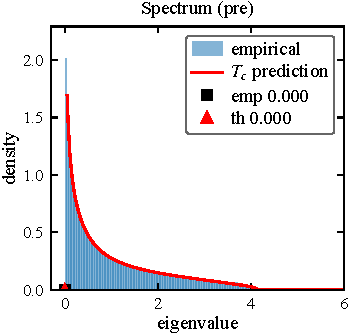
\includegraphics{E1_twopoint_spectrum_pre}%
    \label{fig:e1a}}\hfil
  \subfloat[multinomial]{%
    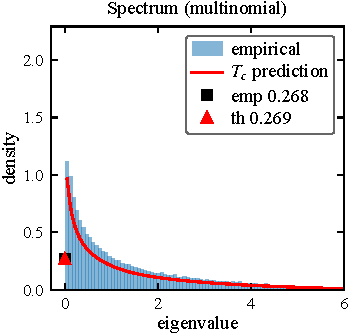
\includegraphics{E1_twopoint_spectrum_multinomial}\label{fig:e1b}}\hfil
  \subfloat[residual]{%
    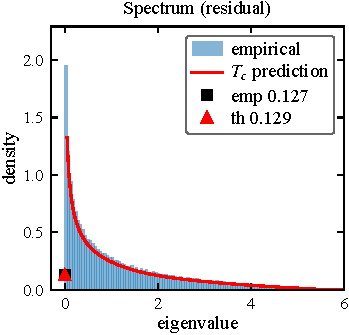
\includegraphics{E1_twopoint_spectrum_residual}\label{fig:e1c}}
  \caption{One map, three count laws: simulated spectra against
    $\mathcal{T}_c$ predictions under the two-point weight law
    $\rho=\tfrac12\delta_{1/2}+\tfrac12\delta_{3/2}$, with an identity
    population and Gaussian entries ($N=1000$, $d=800$, $c=0.8$,
    $n_{\mathrm{rep}}=20$). Zero atoms are drawn as separate point masses at
    the origin and are not merged into the density; all three panels share
    both axes. The three schemes separate as predicted, with second moments
    $2.000$, $2.800$ and $2.400$. The exactly uniform profile is omitted,
    since there residual resampling reproduces the pre-resampling matrix
    itself and the two panels would coincide exactly, which is the content of
    Corollary~\ref{coro:uniform-contrast}; see Table~\ref{tab:e1}. The
    corresponding count probability mass functions are reported in the
    supplementary material~(S.25).}
  \label{fig:e1}
\end{figure*}

% ---------------------------------------------------------------- Table II
\begin{table*}[!t]
\renewcommand{\arraystretch}{1.25}
\caption{Experiment E1: pre-registered spectral quantities against theory.
  Empirical values are means over $n_{\mathrm{rep}}=20$ independent
  repetitions, reported with one standard error. Here $\nu(\{0\})$ denotes the
  count zero mass and $\mu_Q(\{0\})$ the induced spectral atom. Under the
  uniform profile the residual row reproduces the pre-resampling row exactly,
  and not merely to within the reported error. The first spectral moment is
  $1.000$ to within Monte Carlo error in every row and is omitted.}
\label{tab:e1}
\centering
\begin{tabular}{llcccccc}
\toprule
& & \multicolumn{2}{c}{$m_2$}
  & \multicolumn{2}{c}{$\nu(\{0\})$} & \multicolumn{2}{c}{$\mu_Q(\{0\})$} \\
\cmidrule(lr){3-4}\cmidrule(lr){5-6}\cmidrule(lr){7-8}
Profile & Scheme & empirical & theory & empirical & theory
        & empirical & theory \\
\midrule
uniform & pre         & $1.8039\pm0.0012$ & $1.800$
                      & $0$ & $0$ & $0$ & $0$ \\
uniform & multinomial & $2.6118\pm0.0074$ & $2.600$
                      & $0.36805\pm0.00195$ & $0.367879$
                      & $0.21006\pm0.00244$ & $0.209849$ \\
uniform & residual    & $1.8039\pm0.0012$ & $1.800$
                      & $0$ & $0$ & $0$ & $0$ \\
\addlinespace[2pt]
two-point & pre         & $2.0011\pm0.0019$ & $2.000$
                        & $0$ & $0$ & $0$ & $0$ \\
two-point & multinomial & $2.7985\pm0.0103$ & $2.800$
                        & $0.41215\pm0.00230$ & $0.414830$
                        & $0.26519\pm0.00288$ & $0.268538$ \\
two-point & residual    & $2.4026\pm0.0057$ & $2.400$
                        & $0.30580\pm0.00148$ & $0.303265$
                        & $0.13225\pm0.00184$ & $0.129081$ \\
\bottomrule
\end{tabular}
\end{table*}

\emph{Results.} Every pre-registered quantity agrees to within $2\sigma$, and
Table~\ref{tab:e1} reports the full comparison. Two features of the comparison
are not apparent from the tabulated values alone. First, under exactly uniform
weights the residual row does not merely agree with the pre-resampling row to
within the reported error: it reproduces that row exactly, since the realized
matrix is the same, as required by Corollary~\ref{coro:uniform-contrast} at
every finite $N$ and not only in the limit. Second, the Stieltjes
discrepancies at $h=0.05$ have grid means between $0.0019$ and $0.0040$ and
maxima of at most $0.0302$, localized in the left boundary layer; halving the
bandwidth raises the maxima to at most $0.0428$ without altering any
conclusion, which identifies the residual misfit as a boundary-layer effect
rather than a bulk one.

Under the two-point profile the three schemes separate as predicted, with
second moments $2.000$, $2.800$ and $2.400$. Under exactly uniform weights,
multinomial resampling nevertheless produces a zero atom of mass $0.21$. This
distortion is not a small-sample artifact: it is the value predicted by
$\mathcal{T}_c(\operatorname{Poi}(1))$.

The same framework predicts the rank-and-spectral-gap transition at
$c=p_{\mathsf{s}}$ and the conservativeness of the Marchenko--Pastur benchmark
edge, which costs a factor of approximately $1.3$ in the gap it certifies;
both are verified over a twelve-point sweep in $c$ and are reported in the
supplementary material~(S.24).

% ================================================================ IX.D / E3
\subsection{Identical effective sample size with different null spaces}
\label{sec:ix-e3}

Proposition~\ref{prop:ess} states that ESS determines the limiting second
spectral moment given $c$ and $H$, but does not determine the spectrum. The
present experiment quantifies the resulting gap, which is of practical
relevance because ESS is the standard scalar diagnostic for resampling.

\emph{Design.} The pair
\begin{equation}
  \rho^{(A)} = \tfrac12\delta_{1/4}+\tfrac12\delta_{7/4},
  \qquad
  \rho^{(B)} = \tfrac{9}{10}\delta_{3/4}+\tfrac{1}{10}\delta_{13/4}
  \label{eq:e3pair}
\end{equation}
of Proposition~\ref{prop:ess} shares mean $1$ and second moment $25/16$, and
hence shares the value $\mathrm{ESS}=16N/25$ whenever $N$ is a multiple of
$10$, while having distinct count third moments $8.375$ and $9.5$. The
configuration uses multinomial resampling with $c=0.8$, $N=1000$ and
$n_{\mathrm{rep}}=30$. Four quantities are reported: ESS and the predicted
$m_2$, which coincide by construction; the count zero masses; and the spectral
atoms. The count third moments enter through $m_3=1+3cb_2+c^2b_3$.

% ---------------------------------------------------------------- Fig. 3
\begin{figure}[!t]
  \centering
  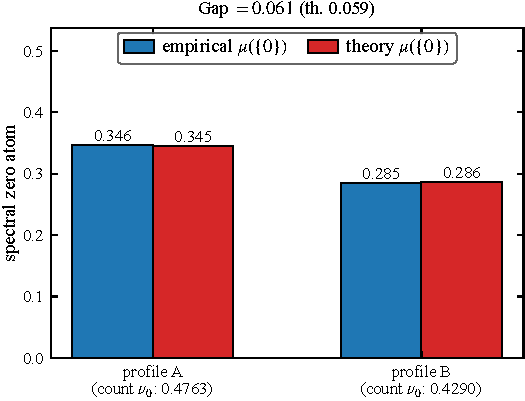
\includegraphics{E3_zero_atom_bars}
  \caption{Two weight profiles with exactly equal ESS, of value $640$, and
    statistically indistinguishable second spectral moments, but
    macroscopically different null spaces, under multinomial resampling with
    $c=0.8$, $N=1000$ and $n_{\mathrm{rep}}=30$. The spectral atoms differ by
    $0.061$ against a pre-registered prediction of $0.059$, a separation of
    nineteen standard errors. Any diagnostic based on ESS reports the two
    configurations as identical.}
  \label{fig:e3}
\end{figure}

% ---------------------------------------------------------------- Table III
\begin{table}[!t]
\renewcommand{\arraystretch}{1.25}
\caption{Experiment E3: identical ESS with different null spaces. Empirical
  values are means over $n_{\mathrm{rep}}=30$ repetitions, reported with one
  standard error. ESS is verified as an exact identity and is not estimated.}
\label{tab:e3}
\centering
\begin{tabular}{lcc}
\toprule
Quantity & Profile $A$ & Profile $B$ \\
\midrule
$\mathrm{ESS}$ (exact)   & $640$ & $640$ \\
$m_2$ empirical          & $3.0559\pm0.0101$ & $3.0397\pm0.0161$ \\
$m_2$ theory             & $3.05$ & $3.05$ \\
$\nu(\{0\})$ empirical   & $0.47717\pm0.00143$ & $0.42823\pm0.00215$ \\
$\nu(\{0\})$ theory      & $0.476287$ & $0.429007$ \\
$\mu_Q(\{0\})$ empirical & $0.34646\pm0.00179$ & $0.28529\pm0.00268$ \\
$\mu_Q(\{0\})$ theory    & $0.345359$ & $0.286259$ \\
$m_3$ empirical          & $12.576\pm0.097$ & $13.171\pm0.180$ \\
$m_3$ theory             & $12.510$ & $13.230$ \\
\bottomrule
\end{tabular}
\end{table}

\emph{Results.} ESS equals $640$ on both sides, verified as an identity
rather than estimated, and the second spectral moments are statistically
indistinguishable, with $|\Delta|=0.0162$ against a joint $2\sigma$ of
$0.0381$. The null spaces are not indistinguishable: the spectral atoms
separate by $0.0612$ against a predicted $0.0591$, or nineteen standard errors,
and the count third moments corroborate the mechanism.
Table~\ref{tab:e3} reports the full comparison.

Two weight configurations that any diagnostic based on ESS reports as identical
therefore differ by six percentage points of the ambient dimension in the
fraction of directions annihilated by a single resampling step. The quantity
involved is finite and directly measurable rather than asymptotic.

% ================================================================ IX.E / E4
\subsection{Residual randomization at the integer boundary}
\label{sec:ix-e4}

\emph{Design.} The three constructions of Theorem~\ref{thm:classification} are
used, all satisfying $\rho_N\Rightarrow\delta_1$: exactly uniform weights,
giving $\alpha=0$; the interior family at $\alpha=0.4$, in which a fraction
$\alpha_N\to\alpha$ of particles is placed at $1-\varepsilon_N$ and the
remainder at $1+\frac{\alpha_N}{1-\alpha_N}\varepsilon_N$, so that
\begin{equation}
  \frac1N\sum_i \lambda_i^2
    = 1 + \frac{\alpha_N}{1-\alpha_N}\varepsilon_N^2,
  \qquad
  \frac{R_N}{N} = \alpha_N;
  \label{eq:e4interior}
\end{equation}
and the bounded two-level endpoint construction $\lambda_i=1-\frac1N$ for
$i<N$ with $\lambda_N=2-\frac1N$ and $N=2^m$, giving $\alpha=1$. Each
construction is run at $N=2^8,\dots,2^{14}$. The reported quantities are
count-level and therefore inexpensive to evaluate: $R_N/N$, the zero-count
fraction, and the second count moment, each compared against the predictions
$\alpha$, $\alpha e^{-1}$ and $1+\alpha$ of
Theorem~\ref{thm:classification} and Proposition~\ref{prop:res-cost}, and
displayed alongside the second-order weight deviation
$\frac1N\sum_i(\lambda_i-1)^2$.

% ---------------------------------------------------------------- Fig. 4
\begin{figure*}[!t]
  \centering
  \subfloat[Second-order weight deviation]{%
    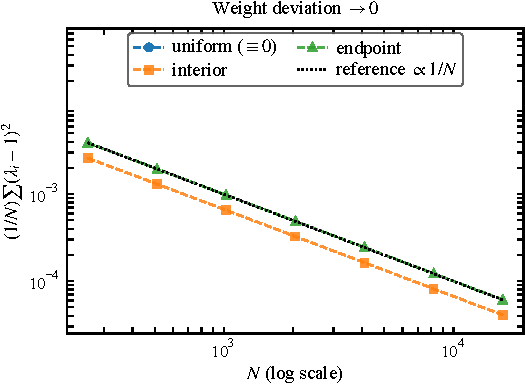
\includegraphics{E4_counts_dev2}\label{fig:e4a}}\hfil
  \subfloat[Residual randomization fraction]{%
    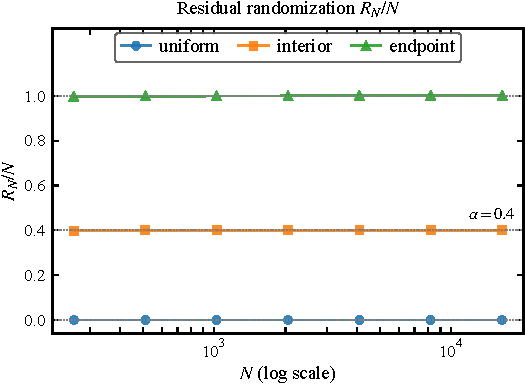
\includegraphics{E4_counts_RnN}\label{fig:e4b}}
  \caption{Vanishing weight heterogeneity does not imply vanishing residual
    randomization, in accordance with Theorem~\ref{thm:classification}.
    \protect\subref{fig:e4a} The second-order deviation
    $\frac1N\sum_i(\lambda_i-1)^2$ vanishes at rate $1/N$ in all three
    constructions, with the dotted line giving the reference slope. The uniform
    construction is omitted from this panel and marked as identically zero in
    the legend, since its deviation vanishes exactly at every $N$ and cannot be
    displayed on a logarithmic axis.
    \protect\subref{fig:e4b} Over the same range, $R_N/N$ converges to the
    three distinct limits $0$, $0.4$ and $1$. The two panels are to be read
    together: the simultaneous vanishing of weight heterogeneity and
    persistence of randomization constitutes the content of
    Theorem~\ref{thm:classification}. Since the endpoint construction keeps
    all weights below $2$, the effect originates in proximity to the integer
    grid rather than in heavy tails.}
  \label{fig:e4}
\end{figure*}

% ---------------------------------------------------------------- Table IV
\begin{table*}[!t]
\renewcommand{\arraystretch}{1.25}
\caption{Experiment E4: count-level quantities for the three constructions of
  Theorem~\ref{thm:classification}, at the endpoints of the sweep; the full
  sweep $N=2^8,\dots,2^{14}$ is tabulated in the supplementary material~(S.26). For
  the uniform construction the counts are
  deterministic, so that all entries are exact and carry no Monte Carlo
  error.}
\label{tab:e4}
\centering
\begin{tabular}{llcccc}
\toprule
Construction & $N$ & $R_N/N$ & zero fraction & $b_{2,N}$
             & $\frac1N\sum(\lambda_i-1)^2$ \\
\midrule
uniform   & all      & $0$ & $0$ & $1$ & $0$ \\
          & (theory) & $0$ & $0$ & $1$ & --- \\
\addlinespace[2pt]
interior  & $256$    & $0.3984$ & $0.15408\pm0.00089$
                     & $1.3963\pm0.0037$ & $2.59\times10^{-3}$ \\
          & $16384$  & $0.4000$ & $0.14835\pm0.00012$
                     & $1.3998\pm0.0005$ & $4.07\times10^{-5}$ \\
          & (theory) & $0.4$    & $0.147152$ & $1.4$ & $\to0$ \\
\addlinespace[2pt]
endpoint  & $256$    & $0.9961$ & $0.36859\pm0.00135$
                     & $2.0034\pm0.0062$ & $3.89\times10^{-3}$ \\
          & $16384$  & $0.9999$ & $0.36800\pm0.00018$
                     & $2.0007\pm0.0008$ & $6.10\times10^{-5}$ \\
          & (theory) & $1$      & $0.367879$ & $2$ & $\to0$ \\
\bottomrule
\end{tabular}
\end{table*}

\emph{Results.} The second-order weight deviation vanishes at rate $1/N$ in
all three constructions: for the interior family it decreases from
$2.59\times10^{-3}$ at $N=256$ to $4.07\times10^{-5}$ at $N=16384$, a factor of
$64$ across a factor of $64$ in $N$. Over the same range $R_N/N$ converges to
the three distinct limits $0$, $0.400$ and $1$, and Table~\ref{tab:e4} reports
the count-level quantities against their predictions $\alpha$, $\alpha e^{-1}$
and $1+\alpha$.

Weight heterogeneity, as measured by any moment of $\rho_N-\delta_1$, may
therefore vanish while residual resampling retains the full randomization of
the multinomial scheme. Since the endpoint construction keeps all weights below
$2$, the effect is governed by the position of the weights relative to the
integer grid and not by heavy tails, and near-uniformity of the weights does
not permit the inference that residual resampling is nearly deterministic.

% ================================================================ IX.F / Fig 5
\subsection{The residual atom-free window}
\label{sec:ix-e4spec}

\emph{Design.} A single spectral configuration of moderate size is used, with
$N=1024$, $d=819$ so that $c=0.7998$, and the interior construction at
$\alpha=0.5$. The pre-resampling, multinomial and residual spectra are
compared against their $\mathcal{T}_c$ predictions. The value $\alpha=0.5$ is
used here in place of the value $\alpha=0.4$ of Fig.~\ref{fig:e4} because it
places $c$ within the window of Corollary~\ref{coro:rank-order} with a wider
margin; the two values yield the same qualitative conclusion.

\emph{Prediction.} At $\alpha=0.5$ the residual count law is
$\tfrac12\delta_1+\tfrac12\operatorname{Poi}(1)$, so that
\begin{equation}
  p_{\mathrm{res}} = 1-\frac{\alpha}{e} = 0.8161,
  \qquad
  p_{\mathrm{multi}} = 1-e^{-1} = 0.6321 .
  \label{eq:e4window}
\end{equation}
With $c=0.7998$ the configuration lies within the window
$c\in(p_{\mathrm{multi}},p_{\mathrm{res}})$ of
Corollary~\ref{coro:rank-order}. The multinomial spectrum must therefore carry
an atom of mass $1-p_{\mathrm{multi}}/c=0.210$, the residual spectrum must
carry none, and the pre-resampling spectrum is $\mathrm{MP}(c)$ without an
atom, since $c<1$.

% ---------------------------------------------------------------- Fig. 5
\begin{figure*}[!t]
  \centering
  \subfloat[pre-resampling]{%
    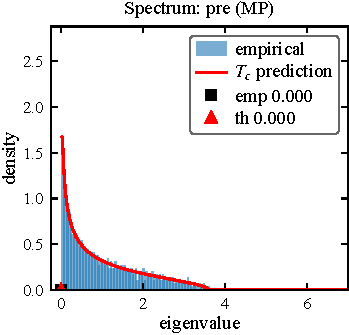
\includegraphics{E4_spectral_pre}\label{fig:e4sa}}\hfil
  \subfloat[multinomial]{%
    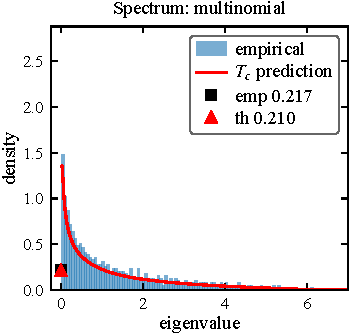
\includegraphics{E4_spectral_multinomial}\label{fig:e4sb}}\hfil
  \subfloat[residual]{%
    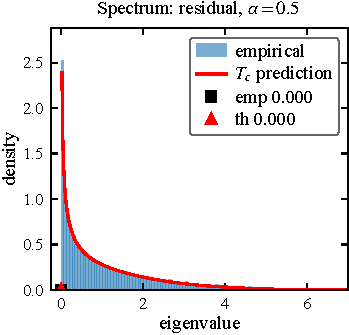
\includegraphics{E4_spectral_residual}\label{fig:e4sc}}
  \caption{The atom-free window of Corollary~\ref{coro:rank-order}, at
    $N=1024$, $d=819$ and $c=0.7998$, with the interior construction at
    $\alpha=0.5$. The value of $\alpha$ differs from that of
    Fig.~\ref{fig:e4}, where $\alpha=0.4$; the larger value places $c$ near
    the centre of the window
    $(p_{\mathrm{multi}},p_{\mathrm{res}})=(0.632,0.816)$. All three panels
    share both axes. \protect\subref{fig:e4sa} The pre-resampling spectrum
    recovers $\mathrm{MP}(c)$. \protect\subref{fig:e4sb} Multinomial
    resampling carries a zero atom of empirical mass $0.217$ against the
    predicted $0.210$. \protect\subref{fig:e4sc} Residual resampling carries
    no atom: within this window it retains full rank with probability tending
    to one, whereas multinomial resampling has already annihilated a fixed
    fraction of directions.}
  \label{fig:e4spec}
\end{figure*}

\emph{Results.} The three panels realize the prediction: the multinomial
spectrum carries an atom of empirical mass $0.217$ against the predicted
$0.210$, the residual spectrum carries none, and the pre-resampling spectrum
recovers $\mathrm{MP}(c)$. Within this window the two schemes differ
qualitatively rather than quantitatively, since multinomial resampling has
already eliminated a fixed fraction of directions while residual resampling
retains full rank with probability tending to one. For $\alpha=0.5$ the window
spans $c\in(0.632,0.816)$, a range that includes many practical ratios of
particle number to dimension.

% ================================================================ IX.G / T1
\subsection{The finite-sample moment identity}
\label{sec:ix-t1}

\emph{Design.} Sections~\ref{sec:lsd}--\ref{sec:res} are asymptotic, whereas
Proposition~\ref{prop:cost} and Corollary~\ref{coro:frob-order} are not, and
are therefore tested separately at a single fixed configuration in which no
limit is taken. One fixed pair $(X,w)$ with $d=150$ and $N=300$, for which the
realized $R_N=124$, is held constant while only the resampling randomness is
redrawn, over $n_{\mathrm{rep}}=1000$ repetitions, for the multinomial and
residual schemes. The residual count covariance is
$\operatorname{Cov}(\bm{n})=\operatorname{diag}(u)-uu^\top/R_N$, with the
branch $R_N=0$ defined to be zero. The cost is evaluated as
\begin{equation}
  \operatorname{tr} S_r^2
    = \frac{1}{N^2}\,\bm{n}^\top (G\circ G)\,\bm{n},
  \label{eq:t1form}
\end{equation}
which requires no eigendecomposition and therefore tests the identity in the
form in which it is proved.

\emph{Results.} At this configuration the standardized deviations are
$1.948$ for multinomial resampling, with Monte Carlo mean $74.114\pm0.520$
against a theoretical cost of $75.128$, and $0.123$ for residual resampling,
with $31.299\pm0.248$ against $31.329$; both lie within the pre-registered
criterion $|\cdot|<3$, so the residual covariance formula is confirmed in the
exact form used in the proof. The covariance difference of
Corollary~\ref{coro:frob-order} is positive semidefinite to machine precision,
with minimum eigenvalue $-2.7\times10^{-15}$, and since $G\circ G\succeq0$ the
finite-sample Frobenius ordering between the two schemes follows. The statement
is conditional and distribution-free, and requires none of the asymptotic
assumptions.

% ================================================================ IX.H
\subsection{Robustness checks}
\label{sec:ix-appendix}

Three checks are summarized here and reported in full in the supplementary
material~(S.27). Repeating the E1 measurements at $N=500$ and $N=2000$ shows every
quantity converging toward its prediction with diminishing error bars, the
uniform-profile count zero mass moving from $0.3646\pm0.0051$ to
$0.3701\pm0.0020$ against $e^{-1}$. Replacing Gaussian entries by variance-one
Rademacher and Student-$t_8$ entries leaves the second spectral moments at
$2.821\pm0.017$ and $2.821\pm0.021$, against the finite-$N$ predictions $2.798$
and $2.801$ of Proposition~\ref{prop:popcost}, which depend on the entry
kurtosis $\kappa_4$; the deviations are $1.3\sigma$ and $0.9\sigma$. This is an
agreement report for a single configuration and is not offered as evidence of
universality, and no universality claim is made in this paper. Finally, for
$H=\tfrac12\delta_{1/2}+\tfrac12\delta_{3/2}$ the separable prediction
$\mu_S=H\boxtimes\mathcal{T}_c(\operatorname{Poi}(1))$ of
Theorem~\ref{thm:lsd-gen} is verified end to end, with post-resampling
$m_2=2.856$ against $2.85$, a zero atom of $0.2079$ against $0.209849$, and the
$\boxtimes$ pipeline matching a directly simulated Wishart spectrum to a
maximum Stieltjes deviation of $5.1\times10^{-4}$.

% =====================================================================

\section{Discussion and Limitations}
\label{sec:limits}

The results above concern four distinct objects, which should not be
conflated\cite{douc2005comparison}: the rank and zero-atom transition, described by $\mu(\{0\})$ with
threshold $p_{\mathsf{s}}$; the universal Marchenko--Pastur lower-edge
benchmark $|\sqrt c-\sqrt{p_{\mathsf{s}}}|^2$; the regular lower and internal
spectral edges, characterized by a branch-restricted critical equation; and
two notions of conditioning, namely the raw pseudo-condition number
$\kappa^+(S)$ and the bulk quantile condition number
\begin{equation}
  \kappa_{\alpha,\beta}^{\mathrm{bulk}}
    :=Q_{\mu^+}(\beta)/Q_{\mu^+}(\alpha),\qquad 0<\alpha<\beta<1,
  \label{eq:bulkcond}
\end{equation}
where $\mu^+:=\mu|_{(0,\infty)}/(1-\mu(\{0\}))$.

The scope of the two conditioning notions depends on the mechanism. For
multinomial resampling in the identity-population model the limiting right
support is unbounded by Proposition~\ref{prop:edges} and
$\kappa^+(S_{r,N})\to\infty$ in probability, since
$\lambda_{\max}(S_{r,N})\to\infty$ while
$\lambda_{\min}^+(S_{r,N})=O_{\mathbb P}(1)$. Fixed-quantile ratios therefore
describe bulk conditioning more robustly than the raw pseudo-condition number,
and a positive lower gap does not imply asymptotic well-conditioning. Residual
limits may instead have bounded support, as in the exact-uniform-weight case,
where $\kappa^+$ has a finite limit for $c\neq1$. The spectral cost considered
in this paper refers to these specific observables and not to generic
performance metrics: given $c$ and $H$, ESS determines the multinomial
limiting second spectral moment and bounds occupancy from below, but does not
determine the full limiting spectral distribution.

Five limitations delimit the scope of the results.

First, the analysis treats a single resampling step with exogenous weights.
Endogenous, likelihood-driven weights generally invalidate the independence
assumptions used in the covariance-spectrum step, so the spectral-map argument
does not extend automatically to that setting. Conditionally on the realized
weights the multinomial sampling law is unchanged, so suitable count-law
limits may survive under corresponding random-weight assumptions.

Second, the limit theorems cover multinomial resampling under (A4) and
residual resampling under (A4R). Establishing count-law limits for stratified
and systematic resampling requires additional analysis of ordering and
dependence and lies outside the scope of this paper; a random-ordering
assumption may prove useful, but is not claimed to be sufficient. These two
schemes accordingly do not appear in the numerical study.

Third, centering is not performed. It perturbs each matrix by a term of rank
at most one and therefore does not affect the limiting spectral distribution
as $d\to\infty$ whenever that distribution exists, but the finite-sample
conditional inequalities are sensitive to it.

Fourth, Theorem~\ref{thm:lsd-gen} is stated under Gaussianity alone, and no
universality claim is made; the entry-distribution check of
Section~\ref{sec:ix-appendix} covers a single configuration and is not a
universality result.

Fifth, the results establish no ordering of filtering accuracy, closed-loop
performance, or optimal resampling schedules: the experiments verify the
objects that the theory defines and no others. The critical-point readings in
Fig.~\ref{fig:e4spec} are finite-$N$ measurements taken near a transition, and
are reported together with their finite-size band rather than smoothed. The
spectral recursion of a complete filtering cycle remains for future work.


\section{Conclusion}
\label{sec:conclusion}

Resampling mechanisms admit a classification by their count-law limits.
Multinomial resampling is determined by the weight law $\rho$ alone, whereas
residual resampling retains information about the approach to the integer
boundaries through the joint law $\pi$, classified completely under
$\rho=\delta_1$ as the family
$(1-\alpha)\delta_1+\alpha\operatorname{Poi}(1)$. Vanishing weight
heterogeneity therefore does not imply vanishing residual randomization.

Composed with a classical covariance-side spectral map, these count laws yield
exact spectral consequences. For multinomial resampling in the
identity-population model they yield a rank-and-spectral-gap transition with
critical support touching, computable regular spectral edges, unbounded right
support with diverging pseudo-condition number, and an exact second-moment
cost. For residual resampling they yield the smaller cost
$c\,a_1^2\,\mathbb{E}_\pi U$, an asymptotic rank-preservation ordering, and a
complete one-parameter classification of the limits under vanishing
heterogeneity. Numerical experiments against pre-registered predictions
confirm each level of the theory.

These results support the use of spectral diagnostics alongside ESS in the
assessment of resampling for high-dimensional ensembles. Their incorporation
into adaptive resampling rules for likelihood-driven particle filters remains
an important direction for future work.

\bibliographystyle{IEEEtran}
\bibliography{dm_refs} 

\end{document}


